% Created by tikzDevice version 0.12.3.1 on 2022-09-05 08:11:24
% !TEX encoding = UTF-8 Unicode
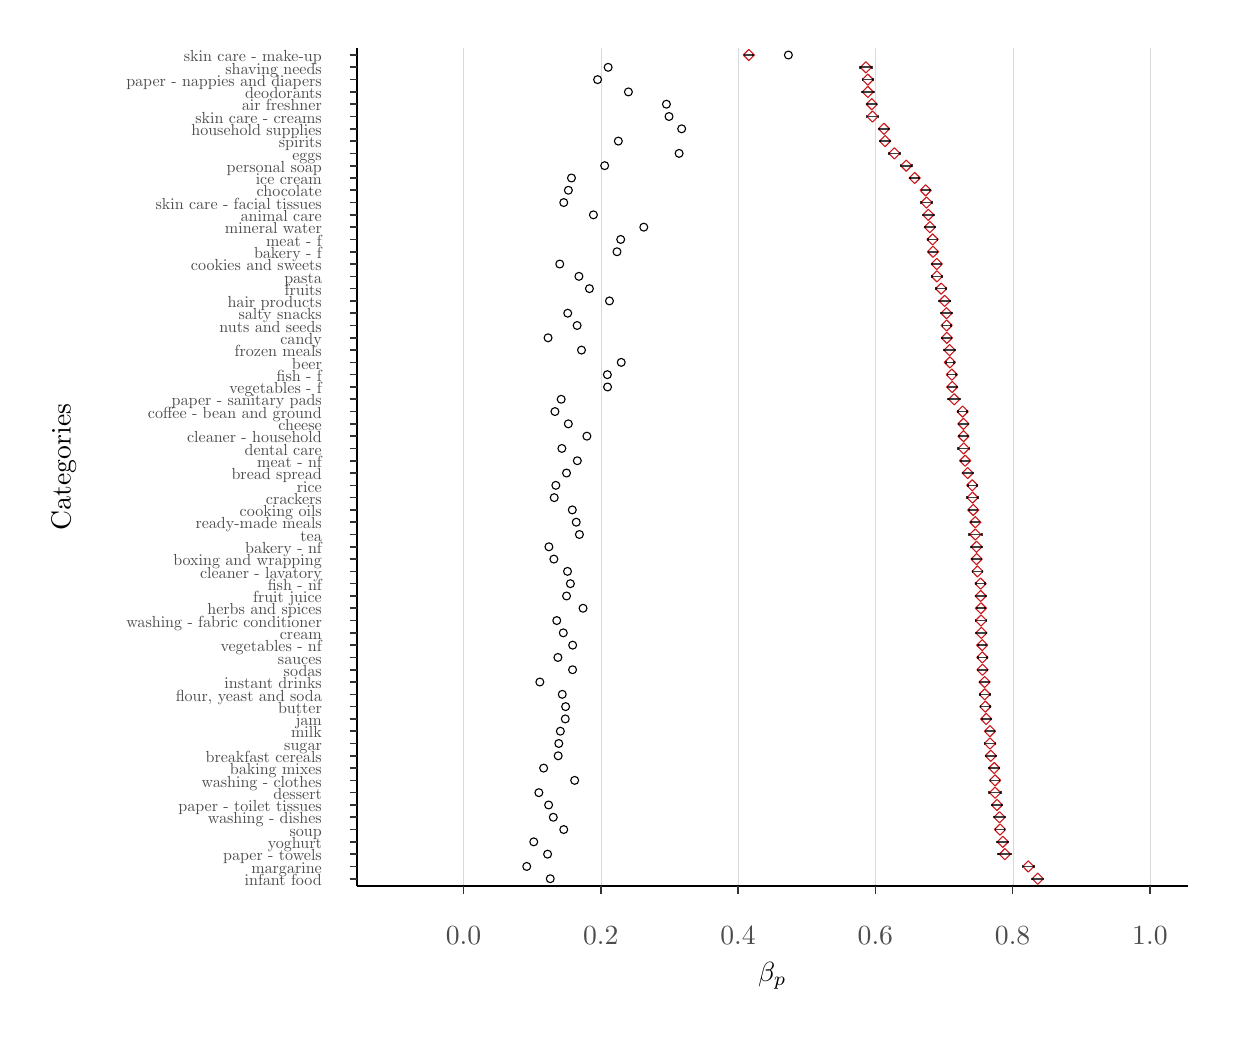
\begin{tikzpicture}[x=1pt,y=1pt]
\definecolor{fillColor}{RGB}{255,255,255}
\path[use as bounding box,fill=fillColor,fill opacity=0.00] (0,0) rectangle (433.62,361.35);
\begin{scope}
\path[clip] (  0.00,  0.00) rectangle (433.62,361.35);
\definecolor{drawColor}{RGB}{255,255,255}
\definecolor{fillColor}{RGB}{255,255,255}

\path[draw=drawColor,line width= 0.6pt,line join=round,line cap=round,fill=fillColor] (  0.00,  0.00) rectangle (433.62,361.35);
\end{scope}
\begin{scope}
\path[clip] (119.04, 51.15) rectangle (419.17,354.12);
\definecolor{drawColor}{RGB}{255,255,255}

\path[draw=drawColor,line width= 0.3pt,line join=round] (132.68, 51.15) --
	(132.68,354.12);

\path[draw=drawColor,line width= 0.3pt,line join=round] (182.29, 51.15) --
	(182.29,354.12);

\path[draw=drawColor,line width= 0.3pt,line join=round] (231.90, 51.15) --
	(231.90,354.12);

\path[draw=drawColor,line width= 0.3pt,line join=round] (281.51, 51.15) --
	(281.51,354.12);

\path[draw=drawColor,line width= 0.3pt,line join=round] (331.11, 51.15) --
	(331.11,354.12);

\path[draw=drawColor,line width= 0.3pt,line join=round] (380.72, 51.15) --
	(380.72,354.12);
\definecolor{drawColor}{gray}{0.85}

\path[draw=drawColor,line width= 0.1pt,line join=round] (157.49, 51.15) --
	(157.49,354.12);

\path[draw=drawColor,line width= 0.1pt,line join=round] (207.09, 51.15) --
	(207.09,354.12);

\path[draw=drawColor,line width= 0.1pt,line join=round] (256.70, 51.15) --
	(256.70,354.12);

\path[draw=drawColor,line width= 0.1pt,line join=round] (306.31, 51.15) --
	(306.31,354.12);

\path[draw=drawColor,line width= 0.1pt,line join=round] (355.92, 51.15) --
	(355.92,354.12);

\path[draw=drawColor,line width= 0.1pt,line join=round] (405.52, 51.15) --
	(405.52,354.12);
\definecolor{drawColor}{RGB}{0,0,0}

\path[draw=drawColor,line width= 0.4pt,line join=round,line cap=round] (230.81,333.69) circle (  1.43);

\path[draw=drawColor,line width= 0.4pt,line join=round,line cap=round] (204.43,293.71) circle (  1.43);

\path[draw=drawColor,line width= 0.4pt,line join=round,line cap=round] (212.95,280.38) circle (  1.43);

\path[draw=drawColor,line width= 0.4pt,line join=round,line cap=round] (188.35,173.76) circle (  1.43);

\path[draw=drawColor,line width= 0.4pt,line join=round,line cap=round] (186.44, 93.80) circle (  1.43);

\path[draw=drawColor,line width= 0.4pt,line join=round,line cap=round] (214.48,240.40) circle (  1.43);

\path[draw=drawColor,line width= 0.4pt,line join=round,line cap=round] (190.14,169.32) circle (  1.43);

\path[draw=drawColor,line width= 0.4pt,line join=round,line cap=round] (194.71,200.42) circle (  1.43);

\path[draw=drawColor,line width= 0.4pt,line join=round,line cap=round] (191.70, 98.24) circle (  1.43);

\path[draw=drawColor,line width= 0.4pt,line join=round,line cap=round] (194.38,116.01) circle (  1.43);

\path[draw=drawColor,line width= 0.4pt,line join=round,line cap=round] (188.04,249.28) circle (  1.43);

\path[draw=drawColor,line width= 0.4pt,line join=round,line cap=round] (195.36,218.19) circle (  1.43);

\path[draw=drawColor,line width= 0.4pt,line join=round,line cap=round] (195.38,302.59) circle (  1.43);

\path[draw=drawColor,line width= 0.4pt,line join=round,line cap=round] (202.07,213.74) circle (  1.43);

\path[draw=drawColor,line width= 0.4pt,line join=round,line cap=round] (195.07,164.88) circle (  1.43);

\path[draw=drawColor,line width= 0.4pt,line join=round,line cap=round] (190.53,222.63) circle (  1.43);

\path[draw=drawColor,line width= 0.4pt,line join=round,line cap=round] (192.27,275.94) circle (  1.43);

\path[draw=drawColor,line width= 0.4pt,line join=round,line cap=round] (196.80,187.09) circle (  1.43);

\path[draw=drawColor,line width= 0.4pt,line join=round,line cap=round] (190.26,191.53) circle (  1.43);

\path[draw=drawColor,line width= 0.4pt,line join=round,line cap=round] (193.54,142.67) circle (  1.43);

\path[draw=drawColor,line width= 0.4pt,line join=round,line cap=round] (193.03,209.30) circle (  1.43);

\path[draw=drawColor,line width= 0.4pt,line join=round,line cap=round] (217.07,338.13) circle (  1.43);

\path[draw=drawColor,line width= 0.4pt,line join=round,line cap=round] (184.72, 84.92) circle (  1.43);

\path[draw=drawColor,line width= 0.4pt,line join=round,line cap=round] (235.39,315.92) circle (  1.43);

\path[draw=drawColor,line width= 0.4pt,line join=round,line cap=round] (209.47,235.96) circle (  1.43);

\path[draw=drawColor,line width= 0.4pt,line join=round,line cap=round] (196.11,160.44) circle (  1.43);

\path[draw=drawColor,line width= 0.4pt,line join=round,line cap=round] (193.17,120.45) circle (  1.43);

\path[draw=drawColor,line width= 0.4pt,line join=round,line cap=round] (200.12,244.84) circle (  1.43);

\path[draw=drawColor,line width= 0.4pt,line join=round,line cap=round] (194.72,155.99) circle (  1.43);

\path[draw=drawColor,line width= 0.4pt,line join=round,line cap=round] (202.99,267.05) circle (  1.43);

\path[draw=drawColor,line width= 0.4pt,line join=round,line cap=round] (210.23,262.61) circle (  1.43);

\path[draw=drawColor,line width= 0.4pt,line join=round,line cap=round] (200.68,151.55) circle (  1.43);

\path[draw=drawColor,line width= 0.4pt,line join=round,line cap=round] (236.32,324.80) circle (  1.43);

\path[draw=drawColor,line width= 0.4pt,line join=round,line cap=round] (196.50,307.03) circle (  1.43);

\path[draw=drawColor,line width= 0.4pt,line join=round,line cap=round] (188.83, 53.82) circle (  1.43);

\path[draw=drawColor,line width= 0.4pt,line join=round,line cap=round] (185.07,124.90) circle (  1.43);

\path[draw=drawColor,line width= 0.4pt,line join=round,line cap=round] (194.26,111.57) circle (  1.43);

\path[draw=drawColor,line width= 0.4pt,line join=round,line cap=round] (180.33, 58.26) circle (  1.43);

\path[draw=drawColor,line width= 0.4pt,line join=round,line cap=round] (214.29,284.82) circle (  1.43);

\path[draw=drawColor,line width= 0.4pt,line join=round,line cap=round] (198.61,204.86) circle (  1.43);

\path[draw=drawColor,line width= 0.4pt,line join=round,line cap=round] (192.48,107.13) circle (  1.43);

\path[draw=drawColor,line width= 0.4pt,line join=round,line cap=round] (222.63,289.26) circle (  1.43);

\path[draw=drawColor,line width= 0.4pt,line join=round,line cap=round] (198.54,253.73) circle (  1.43);

\path[draw=drawColor,line width= 0.4pt,line join=round,line cap=round] (205.94,342.57) circle (  1.43);

\path[draw=drawColor,line width= 0.4pt,line join=round,line cap=round] (192.78,227.07) circle (  1.43);

\path[draw=drawColor,line width= 0.4pt,line join=round,line cap=round] (188.24, 80.47) circle (  1.43);

\path[draw=drawColor,line width= 0.4pt,line join=round,line cap=round] (187.87, 62.70) circle (  1.43);

\path[draw=drawColor,line width= 0.4pt,line join=round,line cap=round] (199.19,271.49) circle (  1.43);

\path[draw=drawColor,line width= 0.4pt,line join=round,line cap=round] (208.50,311.48) circle (  1.43);

\path[draw=drawColor,line width= 0.4pt,line join=round,line cap=round] (198.22,182.65) circle (  1.43);

\path[draw=drawColor,line width= 0.4pt,line join=round,line cap=round] (190.85,195.97) circle (  1.43);

\path[draw=drawColor,line width= 0.4pt,line join=round,line cap=round] (195.15,258.17) circle (  1.43);

\path[draw=drawColor,line width= 0.4pt,line join=round,line cap=round] (191.60,133.78) circle (  1.43);

\path[draw=drawColor,line width= 0.4pt,line join=round,line cap=round] (209.75,347.02) circle (  1.43);

\path[draw=drawColor,line width= 0.4pt,line join=round,line cap=round] (231.75,329.25) circle (  1.43);

\path[draw=drawColor,line width= 0.4pt,line join=round,line cap=round] (193.71,298.15) circle (  1.43);

\path[draw=drawColor,line width= 0.4pt,line join=round,line cap=round] (274.88,351.46) circle (  1.43);

\path[draw=drawColor,line width= 0.4pt,line join=round,line cap=round] (196.90,129.34) circle (  1.43);

\path[draw=drawColor,line width= 0.4pt,line join=round,line cap=round] (193.71, 71.59) circle (  1.43);

\path[draw=drawColor,line width= 0.4pt,line join=round,line cap=round] (213.43,320.36) circle (  1.43);

\path[draw=drawColor,line width= 0.4pt,line join=round,line cap=round] (191.92,102.69) circle (  1.43);

\path[draw=drawColor,line width= 0.4pt,line join=round,line cap=round] (199.37,178.21) circle (  1.43);

\path[draw=drawColor,line width= 0.4pt,line join=round,line cap=round] (209.54,231.51) circle (  1.43);

\path[draw=drawColor,line width= 0.4pt,line join=round,line cap=round] (196.93,138.22) circle (  1.43);

\path[draw=drawColor,line width= 0.4pt,line join=round,line cap=round] (197.65, 89.36) circle (  1.43);

\path[draw=drawColor,line width= 0.4pt,line join=round,line cap=round] (189.93, 76.03) circle (  1.43);

\path[draw=drawColor,line width= 0.4pt,line join=round,line cap=round] (191.18,147.11) circle (  1.43);

\path[draw=drawColor,line width= 0.4pt,line join=round,line cap=round] (182.87, 67.15) circle (  1.43);
\definecolor{drawColor}{RGB}{203,24,29}

\path[draw=drawColor,line width= 0.4pt,line join=round,line cap=round] (303.00,333.69) --
	(305.02,335.71) --
	(307.04,333.69) --
	(305.02,331.67) --
	cycle;

\path[draw=drawColor,line width= 0.4pt,line join=round,line cap=round] (323.43,293.71) --
	(325.45,295.72) --
	(327.47,293.71) --
	(325.45,291.69) --
	cycle;

\path[draw=drawColor,line width= 0.4pt,line join=round,line cap=round] (325.14,280.38) --
	(327.15,282.40) --
	(329.17,280.38) --
	(327.15,278.36) --
	cycle;

\path[draw=drawColor,line width= 0.4pt,line join=round,line cap=round] (340.84,173.76) --
	(342.86,175.78) --
	(344.87,173.76) --
	(342.86,171.75) --
	cycle;

\path[draw=drawColor,line width= 0.4pt,line join=round,line cap=round] (347.24, 93.80) --
	(349.26, 95.82) --
	(351.28, 93.80) --
	(349.26, 91.78) --
	cycle;

\path[draw=drawColor,line width= 0.4pt,line join=round,line cap=round] (331.24,240.40) --
	(333.26,242.42) --
	(335.28,240.40) --
	(333.26,238.38) --
	cycle;

\path[draw=drawColor,line width= 0.4pt,line join=round,line cap=round] (340.88,169.32) --
	(342.89,171.34) --
	(344.91,169.32) --
	(342.89,167.30) --
	cycle;

\path[draw=drawColor,line width= 0.4pt,line join=round,line cap=round] (337.64,200.42) --
	(339.66,202.43) --
	(341.67,200.42) --
	(339.66,198.40) --
	cycle;

\path[draw=drawColor,line width= 0.4pt,line join=round,line cap=round] (346.01, 98.24) --
	(348.02,100.26) --
	(350.04, 98.24) --
	(348.02, 96.23) --
	cycle;

\path[draw=drawColor,line width= 0.4pt,line join=round,line cap=round] (344.01,116.01) --
	(346.03,118.03) --
	(348.05,116.01) --
	(346.03,113.99) --
	cycle;

\path[draw=drawColor,line width= 0.4pt,line join=round,line cap=round] (330.12,249.28) --
	(332.14,251.30) --
	(334.15,249.28) --
	(332.14,247.27) --
	cycle;

\path[draw=drawColor,line width= 0.4pt,line join=round,line cap=round] (336.12,218.19) --
	(338.14,220.20) --
	(340.16,218.19) --
	(338.14,216.17) --
	cycle;

\path[draw=drawColor,line width= 0.4pt,line join=round,line cap=round] (322.46,302.59) --
	(324.47,304.61) --
	(326.49,302.59) --
	(324.47,300.57) --
	cycle;

\path[draw=drawColor,line width= 0.4pt,line join=round,line cap=round] (336.14,213.74) --
	(338.16,215.76) --
	(340.17,213.74) --
	(338.16,211.73) --
	cycle;

\path[draw=drawColor,line width= 0.4pt,line join=round,line cap=round] (341.20,164.88) --
	(343.21,166.90) --
	(345.23,164.88) --
	(343.21,162.86) --
	cycle;

\path[draw=drawColor,line width= 0.4pt,line join=round,line cap=round] (335.82,222.63) --
	(337.84,224.65) --
	(339.86,222.63) --
	(337.84,220.61) --
	cycle;

\path[draw=drawColor,line width= 0.4pt,line join=round,line cap=round] (326.47,275.94) --
	(328.49,277.95) --
	(330.51,275.94) --
	(328.49,273.92) --
	cycle;

\path[draw=drawColor,line width= 0.4pt,line join=round,line cap=round] (339.67,187.09) --
	(341.69,189.11) --
	(343.70,187.09) --
	(341.69,185.07) --
	cycle;

\path[draw=drawColor,line width= 0.4pt,line join=round,line cap=round] (339.42,191.53) --
	(341.43,193.55) --
	(343.45,191.53) --
	(341.43,189.51) --
	cycle;

\path[draw=drawColor,line width= 0.4pt,line join=round,line cap=round] (342.59,142.67) --
	(344.61,144.68) --
	(346.63,142.67) --
	(344.61,140.65) --
	cycle;

\path[draw=drawColor,line width= 0.4pt,line join=round,line cap=round] (336.23,209.30) --
	(338.24,211.32) --
	(340.26,209.30) --
	(338.24,207.28) --
	cycle;

\path[draw=drawColor,line width= 0.4pt,line join=round,line cap=round] (301.57,338.13) --
	(303.59,340.15) --
	(305.61,338.13) --
	(303.59,336.11) --
	cycle;

\path[draw=drawColor,line width= 0.4pt,line join=round,line cap=round] (347.54, 84.92) --
	(349.56, 86.93) --
	(351.58, 84.92) --
	(349.56, 82.90) --
	cycle;

\path[draw=drawColor,line width= 0.4pt,line join=round,line cap=round] (311.15,315.92) --
	(313.17,317.94) --
	(315.18,315.92) --
	(313.17,313.90) --
	cycle;

\path[draw=drawColor,line width= 0.4pt,line join=round,line cap=round] (331.93,235.96) --
	(333.95,237.97) --
	(335.96,235.96) --
	(333.95,233.94) --
	cycle;

\path[draw=drawColor,line width= 0.4pt,line join=round,line cap=round] (342.31,160.44) --
	(344.33,162.45) --
	(346.34,160.44) --
	(344.33,158.42) --
	cycle;

\path[draw=drawColor,line width= 0.4pt,line join=round,line cap=round] (343.83,120.45) --
	(345.84,122.47) --
	(347.86,120.45) --
	(345.84,118.44) --
	cycle;

\path[draw=drawColor,line width= 0.4pt,line join=round,line cap=round] (331.13,244.84) --
	(333.15,246.86) --
	(335.16,244.84) --
	(333.15,242.82) --
	cycle;

\path[draw=drawColor,line width= 0.4pt,line join=round,line cap=round] (342.34,155.99) --
	(344.36,158.01) --
	(346.38,155.99) --
	(344.36,153.98) --
	cycle;

\path[draw=drawColor,line width= 0.4pt,line join=round,line cap=round] (328.08,267.05) --
	(330.10,269.07) --
	(332.12,267.05) --
	(330.10,265.04) --
	cycle;

\path[draw=drawColor,line width= 0.4pt,line join=round,line cap=round] (329.34,262.61) --
	(331.36,264.63) --
	(333.38,262.61) --
	(331.36,260.59) --
	cycle;

\path[draw=drawColor,line width= 0.4pt,line join=round,line cap=round] (342.43,151.55) --
	(344.45,153.57) --
	(346.47,151.55) --
	(344.45,149.53) --
	cycle;

\path[draw=drawColor,line width= 0.4pt,line join=round,line cap=round] (307.40,324.80) --
	(309.42,326.82) --
	(311.44,324.80) --
	(309.42,322.79) --
	cycle;

\path[draw=drawColor,line width= 0.4pt,line join=round,line cap=round] (318.50,307.03) --
	(320.51,309.05) --
	(322.53,307.03) --
	(320.51,305.02) --
	cycle;

\path[draw=drawColor,line width= 0.4pt,line join=round,line cap=round] (362.97, 53.82) --
	(364.98, 55.84) --
	(367.00, 53.82) --
	(364.98, 51.80) --
	cycle;

\path[draw=drawColor,line width= 0.4pt,line join=round,line cap=round] (343.76,124.90) --
	(345.78,126.91) --
	(347.80,124.90) --
	(345.78,122.88) --
	cycle;

\path[draw=drawColor,line width= 0.4pt,line join=round,line cap=round] (344.35,111.57) --
	(346.36,113.59) --
	(348.38,111.57) --
	(346.36,109.55) --
	cycle;

\path[draw=drawColor,line width= 0.4pt,line join=round,line cap=round] (359.56, 58.26) --
	(361.57, 60.28) --
	(363.59, 58.26) --
	(361.57, 56.24) --
	cycle;

\path[draw=drawColor,line width= 0.4pt,line join=round,line cap=round] (324.98,284.82) --
	(327.00,286.84) --
	(329.01,284.82) --
	(327.00,282.80) --
	cycle;

\path[draw=drawColor,line width= 0.4pt,line join=round,line cap=round] (336.72,204.86) --
	(338.74,206.88) --
	(340.76,204.86) --
	(338.74,202.84) --
	cycle;

\path[draw=drawColor,line width= 0.4pt,line join=round,line cap=round] (345.69,107.13) --
	(347.71,109.14) --
	(349.73,107.13) --
	(347.71,105.11) --
	cycle;

\path[draw=drawColor,line width= 0.4pt,line join=round,line cap=round] (323.98,289.26) --
	(326.00,291.28) --
	(328.02,289.26) --
	(326.00,287.25) --
	cycle;

\path[draw=drawColor,line width= 0.4pt,line join=round,line cap=round] (330.05,253.73) --
	(332.07,255.74) --
	(334.08,253.73) --
	(332.07,251.71) --
	cycle;

\path[draw=drawColor,line width= 0.4pt,line join=round,line cap=round] (301.55,342.57) --
	(303.57,344.59) --
	(305.59,342.57) --
	(303.57,340.56) --
	cycle;

\path[draw=drawColor,line width= 0.4pt,line join=round,line cap=round] (332.78,227.07) --
	(334.80,229.09) --
	(336.81,227.07) --
	(334.80,225.05) --
	cycle;

\path[draw=drawColor,line width= 0.4pt,line join=round,line cap=round] (348.23, 80.47) --
	(350.25, 82.49) --
	(352.26, 80.47) --
	(350.25, 78.46) --
	cycle;

\path[draw=drawColor,line width= 0.4pt,line join=round,line cap=round] (351.10, 62.70) --
	(353.12, 64.72) --
	(355.14, 62.70) --
	(353.12, 60.69) --
	cycle;

\path[draw=drawColor,line width= 0.4pt,line join=round,line cap=round] (326.53,271.49) --
	(328.55,273.51) --
	(330.57,271.49) --
	(328.55,269.48) --
	cycle;

\path[draw=drawColor,line width= 0.4pt,line join=round,line cap=round] (315.45,311.48) --
	(317.47,313.49) --
	(319.49,311.48) --
	(317.47,309.46) --
	cycle;

\path[draw=drawColor,line width= 0.4pt,line join=round,line cap=round] (340.40,182.65) --
	(342.41,184.67) --
	(344.43,182.65) --
	(342.41,180.63) --
	cycle;

\path[draw=drawColor,line width= 0.4pt,line join=round,line cap=round] (339.30,195.97) --
	(341.32,197.99) --
	(343.34,195.97) --
	(341.32,193.96) --
	cycle;

\path[draw=drawColor,line width= 0.4pt,line join=round,line cap=round] (330.01,258.17) --
	(332.03,260.19) --
	(334.05,258.17) --
	(332.03,256.15) --
	cycle;

\path[draw=drawColor,line width= 0.4pt,line join=round,line cap=round] (342.95,133.78) --
	(344.97,135.80) --
	(346.98,133.78) --
	(344.97,131.76) --
	cycle;

\path[draw=drawColor,line width= 0.4pt,line join=round,line cap=round] (300.88,347.02) --
	(302.90,349.03) --
	(304.92,347.02) --
	(302.90,345.00) --
	cycle;

\path[draw=drawColor,line width= 0.4pt,line join=round,line cap=round] (303.27,329.25) --
	(305.29,331.26) --
	(307.30,329.25) --
	(305.29,327.23) --
	cycle;

\path[draw=drawColor,line width= 0.4pt,line join=round,line cap=round] (322.77,298.15) --
	(324.79,300.17) --
	(326.81,298.15) --
	(324.79,296.13) --
	cycle;

\path[draw=drawColor,line width= 0.4pt,line join=round,line cap=round] (258.57,351.46) --
	(260.59,353.48) --
	(262.61,351.46) --
	(260.59,349.44) --
	cycle;

\path[draw=drawColor,line width= 0.4pt,line join=round,line cap=round] (343.01,129.34) --
	(345.03,131.36) --
	(347.05,129.34) --
	(345.03,127.32) --
	cycle;

\path[draw=drawColor,line width= 0.4pt,line join=round,line cap=round] (349.34, 71.59) --
	(351.35, 73.61) --
	(353.37, 71.59) --
	(351.35, 69.57) --
	cycle;

\path[draw=drawColor,line width= 0.4pt,line join=round,line cap=round] (307.80,320.36) --
	(309.81,322.38) --
	(311.83,320.36) --
	(309.81,318.34) --
	cycle;

\path[draw=drawColor,line width= 0.4pt,line join=round,line cap=round] (345.73,102.69) --
	(347.74,104.70) --
	(349.76,102.69) --
	(347.74,100.67) --
	cycle;

\path[draw=drawColor,line width= 0.4pt,line join=round,line cap=round] (340.40,178.21) --
	(342.42,180.22) --
	(344.44,178.21) --
	(342.42,176.19) --
	cycle;

\path[draw=drawColor,line width= 0.4pt,line join=round,line cap=round] (332.05,231.51) --
	(334.07,233.53) --
	(336.09,231.51) --
	(334.07,229.50) --
	cycle;

\path[draw=drawColor,line width= 0.4pt,line join=round,line cap=round] (342.90,138.22) --
	(344.92,140.24) --
	(346.93,138.22) --
	(344.92,136.21) --
	cycle;

\path[draw=drawColor,line width= 0.4pt,line join=round,line cap=round] (347.53, 89.36) --
	(349.54, 91.38) --
	(351.56, 89.36) --
	(349.54, 87.34) --
	cycle;

\path[draw=drawColor,line width= 0.4pt,line join=round,line cap=round] (349.16, 76.03) --
	(351.18, 78.05) --
	(353.20, 76.03) --
	(351.18, 74.01) --
	cycle;

\path[draw=drawColor,line width= 0.4pt,line join=round,line cap=round] (342.47,147.11) --
	(344.49,149.13) --
	(346.50,147.11) --
	(344.49,145.09) --
	cycle;

\path[draw=drawColor,line width= 0.4pt,line join=round,line cap=round] (350.35, 67.15) --
	(352.37, 69.16) --
	(354.38, 67.15) --
	(352.37, 65.13) --
	cycle;
\definecolor{drawColor}{RGB}{0,0,0}

\path[draw=drawColor,draw opacity=0.75,line width= 0.6pt,line join=round] (306.74,333.24) --
	(306.74,334.13);

\path[draw=drawColor,draw opacity=0.75,line width= 0.6pt,line join=round] (306.74,333.69) --
	(303.30,333.69);

\path[draw=drawColor,draw opacity=0.75,line width= 0.6pt,line join=round] (303.30,333.24) --
	(303.30,334.13);

\path[draw=drawColor,draw opacity=0.75,line width= 0.6pt,line join=round] (327.51,293.26) --
	(327.51,294.15);

\path[draw=drawColor,draw opacity=0.75,line width= 0.6pt,line join=round] (327.51,293.71) --
	(323.40,293.71);

\path[draw=drawColor,draw opacity=0.75,line width= 0.6pt,line join=round] (323.40,293.26) --
	(323.40,294.15);

\path[draw=drawColor,draw opacity=0.75,line width= 0.6pt,line join=round] (328.80,279.94) --
	(328.80,280.82);

\path[draw=drawColor,draw opacity=0.75,line width= 0.6pt,line join=round] (328.80,280.38) --
	(325.51,280.38);

\path[draw=drawColor,draw opacity=0.75,line width= 0.6pt,line join=round] (325.51,279.94) --
	(325.51,280.82);

\path[draw=drawColor,draw opacity=0.75,line width= 0.6pt,line join=round] (344.84,173.32) --
	(344.84,174.21);

\path[draw=drawColor,draw opacity=0.75,line width= 0.6pt,line join=round] (344.84,173.76) --
	(340.87,173.76);

\path[draw=drawColor,draw opacity=0.75,line width= 0.6pt,line join=round] (340.87,173.32) --
	(340.87,174.21);

\path[draw=drawColor,draw opacity=0.75,line width= 0.6pt,line join=round] (351.18, 93.36) --
	(351.18, 94.24);

\path[draw=drawColor,draw opacity=0.75,line width= 0.6pt,line join=round] (351.18, 93.80) --
	(347.35, 93.80);

\path[draw=drawColor,draw opacity=0.75,line width= 0.6pt,line join=round] (347.35, 93.36) --
	(347.35, 94.24);

\path[draw=drawColor,draw opacity=0.75,line width= 0.6pt,line join=round] (334.77,239.95) --
	(334.77,240.84);

\path[draw=drawColor,draw opacity=0.75,line width= 0.6pt,line join=round] (334.77,240.40) --
	(331.74,240.40);

\path[draw=drawColor,draw opacity=0.75,line width= 0.6pt,line join=round] (331.74,239.95) --
	(331.74,240.84);

\path[draw=drawColor,draw opacity=0.75,line width= 0.6pt,line join=round] (344.68,168.88) --
	(344.68,169.76);

\path[draw=drawColor,draw opacity=0.75,line width= 0.6pt,line join=round] (344.68,169.32) --
	(341.11,169.32);

\path[draw=drawColor,draw opacity=0.75,line width= 0.6pt,line join=round] (341.11,168.88) --
	(341.11,169.76);

\path[draw=drawColor,draw opacity=0.75,line width= 0.6pt,line join=round] (341.49,199.97) --
	(341.49,200.86);

\path[draw=drawColor,draw opacity=0.75,line width= 0.6pt,line join=round] (341.49,200.42) --
	(337.82,200.42);

\path[draw=drawColor,draw opacity=0.75,line width= 0.6pt,line join=round] (337.82,199.97) --
	(337.82,200.86);

\path[draw=drawColor,draw opacity=0.75,line width= 0.6pt,line join=round] (349.96, 97.80) --
	(349.96, 98.69);

\path[draw=drawColor,draw opacity=0.75,line width= 0.6pt,line join=round] (349.96, 98.24) --
	(346.08, 98.24);

\path[draw=drawColor,draw opacity=0.75,line width= 0.6pt,line join=round] (346.08, 97.80) --
	(346.08, 98.69);

\path[draw=drawColor,draw opacity=0.75,line width= 0.6pt,line join=round] (347.81,115.57) --
	(347.81,116.46);

\path[draw=drawColor,draw opacity=0.75,line width= 0.6pt,line join=round] (347.81,116.01) --
	(344.25,116.01);

\path[draw=drawColor,draw opacity=0.75,line width= 0.6pt,line join=round] (344.25,115.57) --
	(344.25,116.46);

\path[draw=drawColor,draw opacity=0.75,line width= 0.6pt,line join=round] (333.85,248.84) --
	(333.85,249.73);

\path[draw=drawColor,draw opacity=0.75,line width= 0.6pt,line join=round] (333.85,249.28) --
	(330.43,249.28);

\path[draw=drawColor,draw opacity=0.75,line width= 0.6pt,line join=round] (330.43,248.84) --
	(330.43,249.73);

\path[draw=drawColor,draw opacity=0.75,line width= 0.6pt,line join=round] (339.92,217.74) --
	(339.92,218.63);

\path[draw=drawColor,draw opacity=0.75,line width= 0.6pt,line join=round] (339.92,218.19) --
	(336.35,218.19);

\path[draw=drawColor,draw opacity=0.75,line width= 0.6pt,line join=round] (336.35,217.74) --
	(336.35,218.63);

\path[draw=drawColor,draw opacity=0.75,line width= 0.6pt,line join=round] (326.01,302.15) --
	(326.01,303.04);

\path[draw=drawColor,draw opacity=0.75,line width= 0.6pt,line join=round] (326.01,302.59) --
	(322.94,302.59);

\path[draw=drawColor,draw opacity=0.75,line width= 0.6pt,line join=round] (322.94,302.15) --
	(322.94,303.04);

\path[draw=drawColor,draw opacity=0.75,line width= 0.6pt,line join=round] (339.81,213.30) --
	(339.81,214.19);

\path[draw=drawColor,draw opacity=0.75,line width= 0.6pt,line join=round] (339.81,213.74) --
	(336.50,213.74);

\path[draw=drawColor,draw opacity=0.75,line width= 0.6pt,line join=round] (336.50,213.30) --
	(336.50,214.19);

\path[draw=drawColor,draw opacity=0.75,line width= 0.6pt,line join=round] (345.02,164.43) --
	(345.02,165.32);

\path[draw=drawColor,draw opacity=0.75,line width= 0.6pt,line join=round] (345.02,164.88) --
	(341.41,164.88);

\path[draw=drawColor,draw opacity=0.75,line width= 0.6pt,line join=round] (341.41,164.43) --
	(341.41,165.32);

\path[draw=drawColor,draw opacity=0.75,line width= 0.6pt,line join=round] (339.53,222.18) --
	(339.53,223.07);

\path[draw=drawColor,draw opacity=0.75,line width= 0.6pt,line join=round] (339.53,222.63) --
	(336.14,222.63);

\path[draw=drawColor,draw opacity=0.75,line width= 0.6pt,line join=round] (336.14,222.18) --
	(336.14,223.07);

\path[draw=drawColor,draw opacity=0.75,line width= 0.6pt,line join=round] (330.15,275.49) --
	(330.15,276.38);

\path[draw=drawColor,draw opacity=0.75,line width= 0.6pt,line join=round] (330.15,275.94) --
	(326.84,275.94);

\path[draw=drawColor,draw opacity=0.75,line width= 0.6pt,line join=round] (326.84,275.49) --
	(326.84,276.38);

\path[draw=drawColor,draw opacity=0.75,line width= 0.6pt,line join=round] (343.17,186.65) --
	(343.17,187.53);

\path[draw=drawColor,draw opacity=0.75,line width= 0.6pt,line join=round] (343.17,187.09) --
	(340.20,187.09);

\path[draw=drawColor,draw opacity=0.75,line width= 0.6pt,line join=round] (340.20,186.65) --
	(340.20,187.53);

\path[draw=drawColor,draw opacity=0.75,line width= 0.6pt,line join=round] (343.40,191.09) --
	(343.40,191.98);

\path[draw=drawColor,draw opacity=0.75,line width= 0.6pt,line join=round] (343.40,191.53) --
	(339.47,191.53);

\path[draw=drawColor,draw opacity=0.75,line width= 0.6pt,line join=round] (339.47,191.09) --
	(339.47,191.98);

\path[draw=drawColor,draw opacity=0.75,line width= 0.6pt,line join=round] (346.51,142.22) --
	(346.51,143.11);

\path[draw=drawColor,draw opacity=0.75,line width= 0.6pt,line join=round] (346.51,142.67) --
	(342.71,142.67);

\path[draw=drawColor,draw opacity=0.75,line width= 0.6pt,line join=round] (342.71,142.22) --
	(342.71,143.11);

\path[draw=drawColor,draw opacity=0.75,line width= 0.6pt,line join=round] (340.30,208.86) --
	(340.30,209.75);

\path[draw=drawColor,draw opacity=0.75,line width= 0.6pt,line join=round] (340.30,209.30) --
	(336.19,209.30);

\path[draw=drawColor,draw opacity=0.75,line width= 0.6pt,line join=round] (336.19,208.86) --
	(336.19,209.75);

\path[draw=drawColor,draw opacity=0.75,line width= 0.6pt,line join=round] (305.70,337.69) --
	(305.70,338.57);

\path[draw=drawColor,draw opacity=0.75,line width= 0.6pt,line join=round] (305.70,338.13) --
	(301.48,338.13);

\path[draw=drawColor,draw opacity=0.75,line width= 0.6pt,line join=round] (301.48,337.69) --
	(301.48,338.57);

\path[draw=drawColor,draw opacity=0.75,line width= 0.6pt,line join=round] (351.73, 84.47) --
	(351.73, 85.36);

\path[draw=drawColor,draw opacity=0.75,line width= 0.6pt,line join=round] (351.73, 84.92) --
	(347.39, 84.92);

\path[draw=drawColor,draw opacity=0.75,line width= 0.6pt,line join=round] (347.39, 84.47) --
	(347.39, 85.36);

\path[draw=drawColor,draw opacity=0.75,line width= 0.6pt,line join=round] (315.11,315.47) --
	(315.11,316.36);

\path[draw=drawColor,draw opacity=0.75,line width= 0.6pt,line join=round] (315.11,315.92) --
	(311.22,315.92);

\path[draw=drawColor,draw opacity=0.75,line width= 0.6pt,line join=round] (311.22,315.47) --
	(311.22,316.36);

\path[draw=drawColor,draw opacity=0.75,line width= 0.6pt,line join=round] (335.54,235.51) --
	(335.54,236.40);

\path[draw=drawColor,draw opacity=0.75,line width= 0.6pt,line join=round] (335.54,235.96) --
	(332.35,235.96);

\path[draw=drawColor,draw opacity=0.75,line width= 0.6pt,line join=round] (332.35,235.51) --
	(332.35,236.40);

\path[draw=drawColor,draw opacity=0.75,line width= 0.6pt,line join=round] (345.95,159.99) --
	(345.95,160.88);

\path[draw=drawColor,draw opacity=0.75,line width= 0.6pt,line join=round] (345.95,160.44) --
	(342.71,160.44);

\path[draw=drawColor,draw opacity=0.75,line width= 0.6pt,line join=round] (342.71,159.99) --
	(342.71,160.88);

\path[draw=drawColor,draw opacity=0.75,line width= 0.6pt,line join=round] (347.67,120.01) --
	(347.67,120.90);

\path[draw=drawColor,draw opacity=0.75,line width= 0.6pt,line join=round] (347.67,120.45) --
	(344.02,120.45);

\path[draw=drawColor,draw opacity=0.75,line width= 0.6pt,line join=round] (344.02,120.01) --
	(344.02,120.90);

\path[draw=drawColor,draw opacity=0.75,line width= 0.6pt,line join=round] (335.19,244.40) --
	(335.19,245.29);

\path[draw=drawColor,draw opacity=0.75,line width= 0.6pt,line join=round] (335.19,244.84) --
	(331.10,244.84);

\path[draw=drawColor,draw opacity=0.75,line width= 0.6pt,line join=round] (331.10,244.40) --
	(331.10,245.29);

\path[draw=drawColor,draw opacity=0.75,line width= 0.6pt,line join=round] (346.20,155.55) --
	(346.20,156.44);

\path[draw=drawColor,draw opacity=0.75,line width= 0.6pt,line join=round] (346.20,155.99) --
	(342.52,155.99);

\path[draw=drawColor,draw opacity=0.75,line width= 0.6pt,line join=round] (342.52,155.55) --
	(342.52,156.44);

\path[draw=drawColor,draw opacity=0.75,line width= 0.6pt,line join=round] (331.88,266.61) --
	(331.88,267.50);

\path[draw=drawColor,draw opacity=0.75,line width= 0.6pt,line join=round] (331.88,267.05) --
	(328.32,267.05);

\path[draw=drawColor,draw opacity=0.75,line width= 0.6pt,line join=round] (328.32,266.61) --
	(328.32,267.50);

\path[draw=drawColor,draw opacity=0.75,line width= 0.6pt,line join=round] (333.47,262.17) --
	(333.47,263.05);

\path[draw=drawColor,draw opacity=0.75,line width= 0.6pt,line join=round] (333.47,262.61) --
	(329.26,262.61);

\path[draw=drawColor,draw opacity=0.75,line width= 0.6pt,line join=round] (329.26,262.17) --
	(329.26,263.05);

\path[draw=drawColor,draw opacity=0.75,line width= 0.6pt,line join=round] (345.98,151.11) --
	(345.98,152.00);

\path[draw=drawColor,draw opacity=0.75,line width= 0.6pt,line join=round] (345.98,151.55) --
	(342.92,151.55);

\path[draw=drawColor,draw opacity=0.75,line width= 0.6pt,line join=round] (342.92,151.11) --
	(342.92,152.00);

\path[draw=drawColor,draw opacity=0.75,line width= 0.6pt,line join=round] (311.18,324.36) --
	(311.18,325.25);

\path[draw=drawColor,draw opacity=0.75,line width= 0.6pt,line join=round] (311.18,324.80) --
	(307.66,324.80);

\path[draw=drawColor,draw opacity=0.75,line width= 0.6pt,line join=round] (307.66,324.36) --
	(307.66,325.25);

\path[draw=drawColor,draw opacity=0.75,line width= 0.6pt,line join=round] (322.16,306.59) --
	(322.16,307.48);

\path[draw=drawColor,draw opacity=0.75,line width= 0.6pt,line join=round] (322.16,307.03) --
	(318.87,307.03);

\path[draw=drawColor,draw opacity=0.75,line width= 0.6pt,line join=round] (318.87,306.59) --
	(318.87,307.48);

\path[draw=drawColor,draw opacity=0.75,line width= 0.6pt,line join=round] (367.02, 53.37) --
	(367.02, 54.26);

\path[draw=drawColor,draw opacity=0.75,line width= 0.6pt,line join=round] (367.02, 53.82) --
	(362.95, 53.82);

\path[draw=drawColor,draw opacity=0.75,line width= 0.6pt,line join=round] (362.95, 53.37) --
	(362.95, 54.26);

\path[draw=drawColor,draw opacity=0.75,line width= 0.6pt,line join=round] (347.57,124.45) --
	(347.57,125.34);

\path[draw=drawColor,draw opacity=0.75,line width= 0.6pt,line join=round] (347.57,124.90) --
	(343.99,124.90);

\path[draw=drawColor,draw opacity=0.75,line width= 0.6pt,line join=round] (343.99,124.45) --
	(343.99,125.34);

\path[draw=drawColor,draw opacity=0.75,line width= 0.6pt,line join=round] (347.98,111.13) --
	(347.98,112.01);

\path[draw=drawColor,draw opacity=0.75,line width= 0.6pt,line join=round] (347.98,111.57) --
	(344.75,111.57);

\path[draw=drawColor,draw opacity=0.75,line width= 0.6pt,line join=round] (344.75,111.13) --
	(344.75,112.01);

\path[draw=drawColor,draw opacity=0.75,line width= 0.6pt,line join=round] (363.65, 57.82) --
	(363.65, 58.71);

\path[draw=drawColor,draw opacity=0.75,line width= 0.6pt,line join=round] (363.65, 58.26) --
	(359.49, 58.26);

\path[draw=drawColor,draw opacity=0.75,line width= 0.6pt,line join=round] (359.49, 57.82) --
	(359.49, 58.71);

\path[draw=drawColor,draw opacity=0.75,line width= 0.6pt,line join=round] (328.74,284.38) --
	(328.74,285.27);

\path[draw=drawColor,draw opacity=0.75,line width= 0.6pt,line join=round] (328.74,284.82) --
	(325.25,284.82);

\path[draw=drawColor,draw opacity=0.75,line width= 0.6pt,line join=round] (325.25,284.38) --
	(325.25,285.27);

\path[draw=drawColor,draw opacity=0.75,line width= 0.6pt,line join=round] (340.29,204.42) --
	(340.29,205.30);

\path[draw=drawColor,draw opacity=0.75,line width= 0.6pt,line join=round] (340.29,204.86) --
	(337.20,204.86);

\path[draw=drawColor,draw opacity=0.75,line width= 0.6pt,line join=round] (337.20,204.42) --
	(337.20,205.30);

\path[draw=drawColor,draw opacity=0.75,line width= 0.6pt,line join=round] (349.37,106.68) --
	(349.37,107.57);

\path[draw=drawColor,draw opacity=0.75,line width= 0.6pt,line join=round] (349.37,107.13) --
	(346.05,107.13);

\path[draw=drawColor,draw opacity=0.75,line width= 0.6pt,line join=round] (346.05,106.68) --
	(346.05,107.57);

\path[draw=drawColor,draw opacity=0.75,line width= 0.6pt,line join=round] (327.88,288.82) --
	(327.88,289.71);

\path[draw=drawColor,draw opacity=0.75,line width= 0.6pt,line join=round] (327.88,289.26) --
	(324.13,289.26);

\path[draw=drawColor,draw opacity=0.75,line width= 0.6pt,line join=round] (324.13,288.82) --
	(324.13,289.71);

\path[draw=drawColor,draw opacity=0.75,line width= 0.6pt,line join=round] (333.58,253.28) --
	(333.58,254.17);

\path[draw=drawColor,draw opacity=0.75,line width= 0.6pt,line join=round] (333.58,253.73) --
	(330.55,253.73);

\path[draw=drawColor,draw opacity=0.75,line width= 0.6pt,line join=round] (330.55,253.28) --
	(330.55,254.17);

\path[draw=drawColor,draw opacity=0.75,line width= 0.6pt,line join=round] (305.45,342.13) --
	(305.45,343.02);

\path[draw=drawColor,draw opacity=0.75,line width= 0.6pt,line join=round] (305.45,342.57) --
	(301.68,342.57);

\path[draw=drawColor,draw opacity=0.75,line width= 0.6pt,line join=round] (301.68,342.13) --
	(301.68,343.02);

\path[draw=drawColor,draw opacity=0.75,line width= 0.6pt,line join=round] (337.04,226.63) --
	(337.04,227.52);

\path[draw=drawColor,draw opacity=0.75,line width= 0.6pt,line join=round] (337.04,227.07) --
	(332.55,227.07);

\path[draw=drawColor,draw opacity=0.75,line width= 0.6pt,line join=round] (332.55,226.63) --
	(332.55,227.52);

\path[draw=drawColor,draw opacity=0.75,line width= 0.6pt,line join=round] (352.04, 80.03) --
	(352.04, 80.92);

\path[draw=drawColor,draw opacity=0.75,line width= 0.6pt,line join=round] (352.04, 80.47) --
	(348.45, 80.47);

\path[draw=drawColor,draw opacity=0.75,line width= 0.6pt,line join=round] (348.45, 80.03) --
	(348.45, 80.92);

\path[draw=drawColor,draw opacity=0.75,line width= 0.6pt,line join=round] (355.49, 62.26) --
	(355.49, 63.15);

\path[draw=drawColor,draw opacity=0.75,line width= 0.6pt,line join=round] (355.49, 62.70) --
	(350.74, 62.70);

\path[draw=drawColor,draw opacity=0.75,line width= 0.6pt,line join=round] (350.74, 62.26) --
	(350.74, 63.15);

\path[draw=drawColor,draw opacity=0.75,line width= 0.6pt,line join=round] (330.28,271.05) --
	(330.28,271.94);

\path[draw=drawColor,draw opacity=0.75,line width= 0.6pt,line join=round] (330.28,271.49) --
	(326.82,271.49);

\path[draw=drawColor,draw opacity=0.75,line width= 0.6pt,line join=round] (326.82,271.05) --
	(326.82,271.94);

\path[draw=drawColor,draw opacity=0.75,line width= 0.6pt,line join=round] (319.50,311.03) --
	(319.50,311.92);

\path[draw=drawColor,draw opacity=0.75,line width= 0.6pt,line join=round] (319.50,311.48) --
	(315.44,311.48);

\path[draw=drawColor,draw opacity=0.75,line width= 0.6pt,line join=round] (315.44,311.03) --
	(315.44,311.92);

\path[draw=drawColor,draw opacity=0.75,line width= 0.6pt,line join=round] (343.92,182.20) --
	(343.92,183.09);

\path[draw=drawColor,draw opacity=0.75,line width= 0.6pt,line join=round] (343.92,182.65) --
	(340.91,182.65);

\path[draw=drawColor,draw opacity=0.75,line width= 0.6pt,line join=round] (340.91,182.20) --
	(340.91,183.09);

\path[draw=drawColor,draw opacity=0.75,line width= 0.6pt,line join=round] (342.97,195.53) --
	(342.97,196.42);

\path[draw=drawColor,draw opacity=0.75,line width= 0.6pt,line join=round] (342.97,195.97) --
	(339.68,195.97);

\path[draw=drawColor,draw opacity=0.75,line width= 0.6pt,line join=round] (339.68,195.53) --
	(339.68,196.42);

\path[draw=drawColor,draw opacity=0.75,line width= 0.6pt,line join=round] (333.96,257.72) --
	(333.96,258.61);

\path[draw=drawColor,draw opacity=0.75,line width= 0.6pt,line join=round] (333.96,258.17) --
	(330.10,258.17);

\path[draw=drawColor,draw opacity=0.75,line width= 0.6pt,line join=round] (330.10,257.72) --
	(330.10,258.61);

\path[draw=drawColor,draw opacity=0.75,line width= 0.6pt,line join=round] (346.65,133.34) --
	(346.65,134.23);

\path[draw=drawColor,draw opacity=0.75,line width= 0.6pt,line join=round] (346.65,133.78) --
	(343.28,133.78);

\path[draw=drawColor,draw opacity=0.75,line width= 0.6pt,line join=round] (343.28,133.34) --
	(343.28,134.23);

\path[draw=drawColor,draw opacity=0.75,line width= 0.6pt,line join=round] (305.16,346.57) --
	(305.16,347.46);

\path[draw=drawColor,draw opacity=0.75,line width= 0.6pt,line join=round] (305.16,347.02) --
	(300.64,347.02);

\path[draw=drawColor,draw opacity=0.75,line width= 0.6pt,line join=round] (300.64,346.57) --
	(300.64,347.46);

\path[draw=drawColor,draw opacity=0.75,line width= 0.6pt,line join=round] (307.41,328.80) --
	(307.41,329.69);

\path[draw=drawColor,draw opacity=0.75,line width= 0.6pt,line join=round] (307.41,329.25) --
	(303.16,329.25);

\path[draw=drawColor,draw opacity=0.75,line width= 0.6pt,line join=round] (303.16,328.80) --
	(303.16,329.69);

\path[draw=drawColor,draw opacity=0.75,line width= 0.6pt,line join=round] (326.82,297.70) --
	(326.82,298.59);

\path[draw=drawColor,draw opacity=0.75,line width= 0.6pt,line join=round] (326.82,298.15) --
	(322.76,298.15);

\path[draw=drawColor,draw opacity=0.75,line width= 0.6pt,line join=round] (322.76,297.70) --
	(322.76,298.59);

\path[draw=drawColor,draw opacity=0.75,line width= 0.6pt,line join=round] (262.13,351.01) --
	(262.13,351.90);

\path[draw=drawColor,draw opacity=0.75,line width= 0.6pt,line join=round] (262.13,351.46) --
	(259.05,351.46);

\path[draw=drawColor,draw opacity=0.75,line width= 0.6pt,line join=round] (259.05,351.01) --
	(259.05,351.90);

\path[draw=drawColor,draw opacity=0.75,line width= 0.6pt,line join=round] (346.87,128.90) --
	(346.87,129.78);

\path[draw=drawColor,draw opacity=0.75,line width= 0.6pt,line join=round] (346.87,129.34) --
	(343.19,129.34);

\path[draw=drawColor,draw opacity=0.75,line width= 0.6pt,line join=round] (343.19,128.90) --
	(343.19,129.78);

\path[draw=drawColor,draw opacity=0.75,line width= 0.6pt,line join=round] (353.00, 71.14) --
	(353.00, 72.03);

\path[draw=drawColor,draw opacity=0.75,line width= 0.6pt,line join=round] (353.00, 71.59) --
	(349.71, 71.59);

\path[draw=drawColor,draw opacity=0.75,line width= 0.6pt,line join=round] (349.71, 71.14) --
	(349.71, 72.03);

\path[draw=drawColor,draw opacity=0.75,line width= 0.6pt,line join=round] (311.68,319.92) --
	(311.68,320.81);

\path[draw=drawColor,draw opacity=0.75,line width= 0.6pt,line join=round] (311.68,320.36) --
	(307.95,320.36);

\path[draw=drawColor,draw opacity=0.75,line width= 0.6pt,line join=round] (307.95,319.92) --
	(307.95,320.81);

\path[draw=drawColor,draw opacity=0.75,line width= 0.6pt,line join=round] (349.73,102.24) --
	(349.73,103.13);

\path[draw=drawColor,draw opacity=0.75,line width= 0.6pt,line join=round] (349.73,102.69) --
	(345.76,102.69);

\path[draw=drawColor,draw opacity=0.75,line width= 0.6pt,line join=round] (345.76,102.24) --
	(345.76,103.13);

\path[draw=drawColor,draw opacity=0.75,line width= 0.6pt,line join=round] (344.73,177.76) --
	(344.73,178.65);

\path[draw=drawColor,draw opacity=0.75,line width= 0.6pt,line join=round] (344.73,178.21) --
	(340.11,178.21);

\path[draw=drawColor,draw opacity=0.75,line width= 0.6pt,line join=round] (340.11,177.76) --
	(340.11,178.65);

\path[draw=drawColor,draw opacity=0.75,line width= 0.6pt,line join=round] (335.78,231.07) --
	(335.78,231.96);

\path[draw=drawColor,draw opacity=0.75,line width= 0.6pt,line join=round] (335.78,231.51) --
	(332.37,231.51);

\path[draw=drawColor,draw opacity=0.75,line width= 0.6pt,line join=round] (332.37,231.07) --
	(332.37,231.96);

\path[draw=drawColor,draw opacity=0.75,line width= 0.6pt,line join=round] (346.40,137.78) --
	(346.40,138.67);

\path[draw=drawColor,draw opacity=0.75,line width= 0.6pt,line join=round] (346.40,138.22) --
	(343.43,138.22);

\path[draw=drawColor,draw opacity=0.75,line width= 0.6pt,line join=round] (343.43,137.78) --
	(343.43,138.67);

\path[draw=drawColor,draw opacity=0.75,line width= 0.6pt,line join=round] (351.16, 88.91) --
	(351.16, 89.80);

\path[draw=drawColor,draw opacity=0.75,line width= 0.6pt,line join=round] (351.16, 89.36) --
	(347.92, 89.36);

\path[draw=drawColor,draw opacity=0.75,line width= 0.6pt,line join=round] (347.92, 88.91) --
	(347.92, 89.80);

\path[draw=drawColor,draw opacity=0.75,line width= 0.6pt,line join=round] (353.28, 75.59) --
	(353.28, 76.48);

\path[draw=drawColor,draw opacity=0.75,line width= 0.6pt,line join=round] (353.28, 76.03) --
	(349.08, 76.03);

\path[draw=drawColor,draw opacity=0.75,line width= 0.6pt,line join=round] (349.08, 75.59) --
	(349.08, 76.48);

\path[draw=drawColor,draw opacity=0.75,line width= 0.6pt,line join=round] (346.50,146.66) --
	(346.50,147.55);

\path[draw=drawColor,draw opacity=0.75,line width= 0.6pt,line join=round] (346.50,147.11) --
	(342.47,147.11);

\path[draw=drawColor,draw opacity=0.75,line width= 0.6pt,line join=round] (342.47,146.66) --
	(342.47,147.55);

\path[draw=drawColor,draw opacity=0.75,line width= 0.6pt,line join=round] (354.35, 66.70) --
	(354.35, 67.59);

\path[draw=drawColor,draw opacity=0.75,line width= 0.6pt,line join=round] (354.35, 67.15) --
	(350.38, 67.15);

\path[draw=drawColor,draw opacity=0.75,line width= 0.6pt,line join=round] (350.38, 66.70) --
	(350.38, 67.59);
\end{scope}
\begin{scope}
\path[clip] (  0.00,  0.00) rectangle (433.62,361.35);
\definecolor{drawColor}{RGB}{0,0,0}

\path[draw=drawColor,line width= 0.6pt,line join=round] (119.04, 51.15) --
	(119.04,354.12);
\end{scope}
\begin{scope}
\path[clip] (  0.00,  0.00) rectangle (433.62,361.35);
\definecolor{drawColor}{gray}{0.30}

\node[text=drawColor,anchor=base east,inner sep=0pt, outer sep=0pt, scale=  0.58] at (106.29, 51.41) {infant food};

\node[text=drawColor,anchor=base east,inner sep=0pt, outer sep=0pt, scale=  0.58] at (106.29, 55.85) {margarine};

\node[text=drawColor,anchor=base east,inner sep=0pt, outer sep=0pt, scale=  0.58] at (106.29, 60.29) {paper - towels};

\node[text=drawColor,anchor=base east,inner sep=0pt, outer sep=0pt, scale=  0.58] at (106.29, 64.74) {yoghurt};

\node[text=drawColor,anchor=base east,inner sep=0pt, outer sep=0pt, scale=  0.58] at (106.29, 69.18) {soup};

\node[text=drawColor,anchor=base east,inner sep=0pt, outer sep=0pt, scale=  0.58] at (106.29, 73.62) {washing - dishes};

\node[text=drawColor,anchor=base east,inner sep=0pt, outer sep=0pt, scale=  0.58] at (106.29, 78.06) {paper - toilet tissues};

\node[text=drawColor,anchor=base east,inner sep=0pt, outer sep=0pt, scale=  0.58] at (106.29, 82.50) {dessert};

\node[text=drawColor,anchor=base east,inner sep=0pt, outer sep=0pt, scale=  0.58] at (106.29, 86.95) {washing - clothes};

\node[text=drawColor,anchor=base east,inner sep=0pt, outer sep=0pt, scale=  0.58] at (106.29, 91.39) {baking mixes};

\node[text=drawColor,anchor=base east,inner sep=0pt, outer sep=0pt, scale=  0.58] at (106.29, 95.83) {breakfast cereals};

\node[text=drawColor,anchor=base east,inner sep=0pt, outer sep=0pt, scale=  0.58] at (106.29,100.27) {sugar};

\node[text=drawColor,anchor=base east,inner sep=0pt, outer sep=0pt, scale=  0.58] at (106.29,104.72) {milk};

\node[text=drawColor,anchor=base east,inner sep=0pt, outer sep=0pt, scale=  0.58] at (106.29,109.16) {jam};

\node[text=drawColor,anchor=base east,inner sep=0pt, outer sep=0pt, scale=  0.58] at (106.29,113.60) {butter};

\node[text=drawColor,anchor=base east,inner sep=0pt, outer sep=0pt, scale=  0.58] at (106.29,118.04) {flour, yeast and soda};

\node[text=drawColor,anchor=base east,inner sep=0pt, outer sep=0pt, scale=  0.58] at (106.29,122.49) {instant drinks};

\node[text=drawColor,anchor=base east,inner sep=0pt, outer sep=0pt, scale=  0.58] at (106.29,126.93) {sodas};

\node[text=drawColor,anchor=base east,inner sep=0pt, outer sep=0pt, scale=  0.58] at (106.29,131.37) {sauces};

\node[text=drawColor,anchor=base east,inner sep=0pt, outer sep=0pt, scale=  0.58] at (106.29,135.81) {vegetables - nf};

\node[text=drawColor,anchor=base east,inner sep=0pt, outer sep=0pt, scale=  0.58] at (106.29,140.26) {cream};

\node[text=drawColor,anchor=base east,inner sep=0pt, outer sep=0pt, scale=  0.58] at (106.29,144.70) {washing - fabric conditioner};

\node[text=drawColor,anchor=base east,inner sep=0pt, outer sep=0pt, scale=  0.58] at (106.29,149.14) {herbs and spices};

\node[text=drawColor,anchor=base east,inner sep=0pt, outer sep=0pt, scale=  0.58] at (106.29,153.58) {fruit juice};

\node[text=drawColor,anchor=base east,inner sep=0pt, outer sep=0pt, scale=  0.58] at (106.29,158.02) {fish - nf};

\node[text=drawColor,anchor=base east,inner sep=0pt, outer sep=0pt, scale=  0.58] at (106.29,162.47) {cleaner - lavatory};

\node[text=drawColor,anchor=base east,inner sep=0pt, outer sep=0pt, scale=  0.58] at (106.29,166.91) {boxing and wrapping};

\node[text=drawColor,anchor=base east,inner sep=0pt, outer sep=0pt, scale=  0.58] at (106.29,171.35) {bakery - nf};

\node[text=drawColor,anchor=base east,inner sep=0pt, outer sep=0pt, scale=  0.58] at (106.29,175.79) {tea};

\node[text=drawColor,anchor=base east,inner sep=0pt, outer sep=0pt, scale=  0.58] at (106.29,180.24) {ready-made meals};

\node[text=drawColor,anchor=base east,inner sep=0pt, outer sep=0pt, scale=  0.58] at (106.29,184.68) {cooking oils};

\node[text=drawColor,anchor=base east,inner sep=0pt, outer sep=0pt, scale=  0.58] at (106.29,189.12) {crackers};

\node[text=drawColor,anchor=base east,inner sep=0pt, outer sep=0pt, scale=  0.58] at (106.29,193.56) {rice};

\node[text=drawColor,anchor=base east,inner sep=0pt, outer sep=0pt, scale=  0.58] at (106.29,198.01) {bread spread};

\node[text=drawColor,anchor=base east,inner sep=0pt, outer sep=0pt, scale=  0.58] at (106.29,202.45) {meat - nf};

\node[text=drawColor,anchor=base east,inner sep=0pt, outer sep=0pt, scale=  0.58] at (106.29,206.89) {dental care};

\node[text=drawColor,anchor=base east,inner sep=0pt, outer sep=0pt, scale=  0.58] at (106.29,211.33) {cleaner - household};

\node[text=drawColor,anchor=base east,inner sep=0pt, outer sep=0pt, scale=  0.58] at (106.29,215.78) {cheese};

\node[text=drawColor,anchor=base east,inner sep=0pt, outer sep=0pt, scale=  0.58] at (106.29,220.22) {coffee - bean and ground};

\node[text=drawColor,anchor=base east,inner sep=0pt, outer sep=0pt, scale=  0.58] at (106.29,224.66) {paper - sanitary pads};

\node[text=drawColor,anchor=base east,inner sep=0pt, outer sep=0pt, scale=  0.58] at (106.29,229.10) {vegetables - f};

\node[text=drawColor,anchor=base east,inner sep=0pt, outer sep=0pt, scale=  0.58] at (106.29,233.55) {fish - f};

\node[text=drawColor,anchor=base east,inner sep=0pt, outer sep=0pt, scale=  0.58] at (106.29,237.99) {beer};

\node[text=drawColor,anchor=base east,inner sep=0pt, outer sep=0pt, scale=  0.58] at (106.29,242.43) {frozen meals};

\node[text=drawColor,anchor=base east,inner sep=0pt, outer sep=0pt, scale=  0.58] at (106.29,246.87) {candy};

\node[text=drawColor,anchor=base east,inner sep=0pt, outer sep=0pt, scale=  0.58] at (106.29,251.31) {nuts and seeds};

\node[text=drawColor,anchor=base east,inner sep=0pt, outer sep=0pt, scale=  0.58] at (106.29,255.76) {salty snacks};

\node[text=drawColor,anchor=base east,inner sep=0pt, outer sep=0pt, scale=  0.58] at (106.29,260.20) {hair products};

\node[text=drawColor,anchor=base east,inner sep=0pt, outer sep=0pt, scale=  0.58] at (106.29,264.64) {fruits};

\node[text=drawColor,anchor=base east,inner sep=0pt, outer sep=0pt, scale=  0.58] at (106.29,269.08) {pasta};

\node[text=drawColor,anchor=base east,inner sep=0pt, outer sep=0pt, scale=  0.58] at (106.29,273.53) {cookies and sweets};

\node[text=drawColor,anchor=base east,inner sep=0pt, outer sep=0pt, scale=  0.58] at (106.29,277.97) {bakery - f};

\node[text=drawColor,anchor=base east,inner sep=0pt, outer sep=0pt, scale=  0.58] at (106.29,282.41) {meat - f};

\node[text=drawColor,anchor=base east,inner sep=0pt, outer sep=0pt, scale=  0.58] at (106.29,286.85) {mineral water};

\node[text=drawColor,anchor=base east,inner sep=0pt, outer sep=0pt, scale=  0.58] at (106.29,291.30) {animal care};

\node[text=drawColor,anchor=base east,inner sep=0pt, outer sep=0pt, scale=  0.58] at (106.29,295.74) {skin care - facial tissues};

\node[text=drawColor,anchor=base east,inner sep=0pt, outer sep=0pt, scale=  0.58] at (106.29,300.18) {chocolate};

\node[text=drawColor,anchor=base east,inner sep=0pt, outer sep=0pt, scale=  0.58] at (106.29,304.62) {ice cream};

\node[text=drawColor,anchor=base east,inner sep=0pt, outer sep=0pt, scale=  0.58] at (106.29,309.07) {personal soap};

\node[text=drawColor,anchor=base east,inner sep=0pt, outer sep=0pt, scale=  0.58] at (106.29,313.51) {eggs};

\node[text=drawColor,anchor=base east,inner sep=0pt, outer sep=0pt, scale=  0.58] at (106.29,317.95) {spirits};

\node[text=drawColor,anchor=base east,inner sep=0pt, outer sep=0pt, scale=  0.58] at (106.29,322.39) {household supplies};

\node[text=drawColor,anchor=base east,inner sep=0pt, outer sep=0pt, scale=  0.58] at (106.29,326.83) {skin care - creams};

\node[text=drawColor,anchor=base east,inner sep=0pt, outer sep=0pt, scale=  0.58] at (106.29,331.28) {air freshner};

\node[text=drawColor,anchor=base east,inner sep=0pt, outer sep=0pt, scale=  0.58] at (106.29,335.72) {deodorants};

\node[text=drawColor,anchor=base east,inner sep=0pt, outer sep=0pt, scale=  0.58] at (106.29,340.16) {paper - nappies and diapers};

\node[text=drawColor,anchor=base east,inner sep=0pt, outer sep=0pt, scale=  0.58] at (106.29,344.60) {shaving needs};

\node[text=drawColor,anchor=base east,inner sep=0pt, outer sep=0pt, scale=  0.58] at (106.29,349.05) {skin care - make-up};
\end{scope}
\begin{scope}
\path[clip] (  0.00,  0.00) rectangle (433.62,361.35);
\definecolor{drawColor}{gray}{0.20}

\path[draw=drawColor,line width= 0.6pt,line join=round] (116.29, 53.82) --
	(119.04, 53.82);

\path[draw=drawColor,line width= 0.6pt,line join=round] (116.29, 58.26) --
	(119.04, 58.26);

\path[draw=drawColor,line width= 0.6pt,line join=round] (116.29, 62.70) --
	(119.04, 62.70);

\path[draw=drawColor,line width= 0.6pt,line join=round] (116.29, 67.15) --
	(119.04, 67.15);

\path[draw=drawColor,line width= 0.6pt,line join=round] (116.29, 71.59) --
	(119.04, 71.59);

\path[draw=drawColor,line width= 0.6pt,line join=round] (116.29, 76.03) --
	(119.04, 76.03);

\path[draw=drawColor,line width= 0.6pt,line join=round] (116.29, 80.47) --
	(119.04, 80.47);

\path[draw=drawColor,line width= 0.6pt,line join=round] (116.29, 84.92) --
	(119.04, 84.92);

\path[draw=drawColor,line width= 0.6pt,line join=round] (116.29, 89.36) --
	(119.04, 89.36);

\path[draw=drawColor,line width= 0.6pt,line join=round] (116.29, 93.80) --
	(119.04, 93.80);

\path[draw=drawColor,line width= 0.6pt,line join=round] (116.29, 98.24) --
	(119.04, 98.24);

\path[draw=drawColor,line width= 0.6pt,line join=round] (116.29,102.69) --
	(119.04,102.69);

\path[draw=drawColor,line width= 0.6pt,line join=round] (116.29,107.13) --
	(119.04,107.13);

\path[draw=drawColor,line width= 0.6pt,line join=round] (116.29,111.57) --
	(119.04,111.57);

\path[draw=drawColor,line width= 0.6pt,line join=round] (116.29,116.01) --
	(119.04,116.01);

\path[draw=drawColor,line width= 0.6pt,line join=round] (116.29,120.45) --
	(119.04,120.45);

\path[draw=drawColor,line width= 0.6pt,line join=round] (116.29,124.90) --
	(119.04,124.90);

\path[draw=drawColor,line width= 0.6pt,line join=round] (116.29,129.34) --
	(119.04,129.34);

\path[draw=drawColor,line width= 0.6pt,line join=round] (116.29,133.78) --
	(119.04,133.78);

\path[draw=drawColor,line width= 0.6pt,line join=round] (116.29,138.22) --
	(119.04,138.22);

\path[draw=drawColor,line width= 0.6pt,line join=round] (116.29,142.67) --
	(119.04,142.67);

\path[draw=drawColor,line width= 0.6pt,line join=round] (116.29,147.11) --
	(119.04,147.11);

\path[draw=drawColor,line width= 0.6pt,line join=round] (116.29,151.55) --
	(119.04,151.55);

\path[draw=drawColor,line width= 0.6pt,line join=round] (116.29,155.99) --
	(119.04,155.99);

\path[draw=drawColor,line width= 0.6pt,line join=round] (116.29,160.44) --
	(119.04,160.44);

\path[draw=drawColor,line width= 0.6pt,line join=round] (116.29,164.88) --
	(119.04,164.88);

\path[draw=drawColor,line width= 0.6pt,line join=round] (116.29,169.32) --
	(119.04,169.32);

\path[draw=drawColor,line width= 0.6pt,line join=round] (116.29,173.76) --
	(119.04,173.76);

\path[draw=drawColor,line width= 0.6pt,line join=round] (116.29,178.21) --
	(119.04,178.21);

\path[draw=drawColor,line width= 0.6pt,line join=round] (116.29,182.65) --
	(119.04,182.65);

\path[draw=drawColor,line width= 0.6pt,line join=round] (116.29,187.09) --
	(119.04,187.09);

\path[draw=drawColor,line width= 0.6pt,line join=round] (116.29,191.53) --
	(119.04,191.53);

\path[draw=drawColor,line width= 0.6pt,line join=round] (116.29,195.97) --
	(119.04,195.97);

\path[draw=drawColor,line width= 0.6pt,line join=round] (116.29,200.42) --
	(119.04,200.42);

\path[draw=drawColor,line width= 0.6pt,line join=round] (116.29,204.86) --
	(119.04,204.86);

\path[draw=drawColor,line width= 0.6pt,line join=round] (116.29,209.30) --
	(119.04,209.30);

\path[draw=drawColor,line width= 0.6pt,line join=round] (116.29,213.74) --
	(119.04,213.74);

\path[draw=drawColor,line width= 0.6pt,line join=round] (116.29,218.19) --
	(119.04,218.19);

\path[draw=drawColor,line width= 0.6pt,line join=round] (116.29,222.63) --
	(119.04,222.63);

\path[draw=drawColor,line width= 0.6pt,line join=round] (116.29,227.07) --
	(119.04,227.07);

\path[draw=drawColor,line width= 0.6pt,line join=round] (116.29,231.51) --
	(119.04,231.51);

\path[draw=drawColor,line width= 0.6pt,line join=round] (116.29,235.96) --
	(119.04,235.96);

\path[draw=drawColor,line width= 0.6pt,line join=round] (116.29,240.40) --
	(119.04,240.40);

\path[draw=drawColor,line width= 0.6pt,line join=round] (116.29,244.84) --
	(119.04,244.84);

\path[draw=drawColor,line width= 0.6pt,line join=round] (116.29,249.28) --
	(119.04,249.28);

\path[draw=drawColor,line width= 0.6pt,line join=round] (116.29,253.73) --
	(119.04,253.73);

\path[draw=drawColor,line width= 0.6pt,line join=round] (116.29,258.17) --
	(119.04,258.17);

\path[draw=drawColor,line width= 0.6pt,line join=round] (116.29,262.61) --
	(119.04,262.61);

\path[draw=drawColor,line width= 0.6pt,line join=round] (116.29,267.05) --
	(119.04,267.05);

\path[draw=drawColor,line width= 0.6pt,line join=round] (116.29,271.49) --
	(119.04,271.49);

\path[draw=drawColor,line width= 0.6pt,line join=round] (116.29,275.94) --
	(119.04,275.94);

\path[draw=drawColor,line width= 0.6pt,line join=round] (116.29,280.38) --
	(119.04,280.38);

\path[draw=drawColor,line width= 0.6pt,line join=round] (116.29,284.82) --
	(119.04,284.82);

\path[draw=drawColor,line width= 0.6pt,line join=round] (116.29,289.26) --
	(119.04,289.26);

\path[draw=drawColor,line width= 0.6pt,line join=round] (116.29,293.71) --
	(119.04,293.71);

\path[draw=drawColor,line width= 0.6pt,line join=round] (116.29,298.15) --
	(119.04,298.15);

\path[draw=drawColor,line width= 0.6pt,line join=round] (116.29,302.59) --
	(119.04,302.59);

\path[draw=drawColor,line width= 0.6pt,line join=round] (116.29,307.03) --
	(119.04,307.03);

\path[draw=drawColor,line width= 0.6pt,line join=round] (116.29,311.48) --
	(119.04,311.48);

\path[draw=drawColor,line width= 0.6pt,line join=round] (116.29,315.92) --
	(119.04,315.92);

\path[draw=drawColor,line width= 0.6pt,line join=round] (116.29,320.36) --
	(119.04,320.36);

\path[draw=drawColor,line width= 0.6pt,line join=round] (116.29,324.80) --
	(119.04,324.80);

\path[draw=drawColor,line width= 0.6pt,line join=round] (116.29,329.25) --
	(119.04,329.25);

\path[draw=drawColor,line width= 0.6pt,line join=round] (116.29,333.69) --
	(119.04,333.69);

\path[draw=drawColor,line width= 0.6pt,line join=round] (116.29,338.13) --
	(119.04,338.13);

\path[draw=drawColor,line width= 0.6pt,line join=round] (116.29,342.57) --
	(119.04,342.57);

\path[draw=drawColor,line width= 0.6pt,line join=round] (116.29,347.02) --
	(119.04,347.02);

\path[draw=drawColor,line width= 0.6pt,line join=round] (116.29,351.46) --
	(119.04,351.46);
\end{scope}
\begin{scope}
\path[clip] (  0.00,  0.00) rectangle (433.62,361.35);
\definecolor{drawColor}{RGB}{0,0,0}

\path[draw=drawColor,line width= 0.6pt,line join=round] (119.04, 51.15) --
	(419.17, 51.15);
\end{scope}
\begin{scope}
\path[clip] (  0.00,  0.00) rectangle (433.62,361.35);
\definecolor{drawColor}{gray}{0.20}

\path[draw=drawColor,line width= 0.6pt,line join=round] (157.49, 48.40) --
	(157.49, 51.15);

\path[draw=drawColor,line width= 0.6pt,line join=round] (207.09, 48.40) --
	(207.09, 51.15);

\path[draw=drawColor,line width= 0.6pt,line join=round] (256.70, 48.40) --
	(256.70, 51.15);

\path[draw=drawColor,line width= 0.6pt,line join=round] (306.31, 48.40) --
	(306.31, 51.15);

\path[draw=drawColor,line width= 0.6pt,line join=round] (355.92, 48.40) --
	(355.92, 51.15);

\path[draw=drawColor,line width= 0.6pt,line join=round] (405.52, 48.40) --
	(405.52, 51.15);
\end{scope}
\begin{scope}
\path[clip] (  0.00,  0.00) rectangle (433.62,361.35);
\definecolor{drawColor}{gray}{0.30}

\node[text=drawColor,anchor=base,inner sep=0pt, outer sep=0pt, scale=  1.00] at (157.49, 30.14) {0.0};

\node[text=drawColor,anchor=base,inner sep=0pt, outer sep=0pt, scale=  1.00] at (207.09, 30.14) {0.2};

\node[text=drawColor,anchor=base,inner sep=0pt, outer sep=0pt, scale=  1.00] at (256.70, 30.14) {0.4};

\node[text=drawColor,anchor=base,inner sep=0pt, outer sep=0pt, scale=  1.00] at (306.31, 30.14) {0.6};

\node[text=drawColor,anchor=base,inner sep=0pt, outer sep=0pt, scale=  1.00] at (355.92, 30.14) {0.8};

\node[text=drawColor,anchor=base,inner sep=0pt, outer sep=0pt, scale=  1.00] at (405.52, 30.14) {1.0};
\end{scope}
\begin{scope}
\path[clip] (  0.00,  0.00) rectangle (433.62,361.35);
\definecolor{drawColor}{RGB}{0,0,0}

\node[text=drawColor,anchor=base,inner sep=0pt, outer sep=0pt, scale=  1.00] at (269.10, 16.79) {$\beta_{p}$};
\end{scope}
\begin{scope}
\path[clip] (  0.00,  0.00) rectangle (433.62,361.35);
\definecolor{drawColor}{RGB}{0,0,0}

\node[text=drawColor,rotate= 90.00,anchor=base,inner sep=0pt, outer sep=0pt, scale=  1.00] at ( 15.49,202.64) {Categories};
\end{scope}
\end{tikzpicture}
